\documentclass[a4paper,12pt]{report}

\usepackage{alltt, fancyvrb, url}
\usepackage{graphicx}
\usepackage[utf8]{inputenc}
\usepackage{float}
\usepackage{xcolor}
\usepackage{hyperref}

% Questo commentalo se vuoi scrivere in inglese.
\usepackage[italian]{babel}

\usepackage[italian]{cleveref}

\title{Make an Ice Cream}

\author{Chiara Emina, Sophy Mercuri, Antonio Scharmuller, Shuyi Zhang}
\date{\today}


\begin{document}

\maketitle

\tableofcontents

\chapter{Analisi}

\section{Descrizione e requisiti}

Il software oggetto di questo progetto è un videogioco intitolato 'Make an Ice Cream'. L'obiettivo dell’applicazione è quello di offrire un’esperienza di gioco, in cui l’utente assume il ruolo di un gelatiere che deve soddisfare gli ordini di una serie di clienti entro dei vincoli temporali prestabiliti. Durante lo svolgimento del gioco, all’utente vengono presentati diversi clienti in modo sequenziale, uno alla volta, e ognuno è caratterizzato da un ordine specifico e da un timer. L’ordine di un cliente descrive la composizione del gelato desiderato, e il timer specifica il tempo limite entro il quale l’ordine deve essere completato. Al giocatore vengono inoltre forniti, su un bancone, una serie di ingredienti quali gusti di gelato, tipi di cono e topping. Il compito del giocatore è quello di selezionare gli ingredienti appropriati e comporre il gelato in modo conforme all’ordine, per poi consegnarlo al cliente. Il gioco è strutturato in livelli a difficoltà crescente: con l’avanzare dei livelli aumentano la complessità degli ordini e il numero complessivo di clienti, e diminuisce il tempo limite di ciascun cliente. Inoltre, il sistema prevede un numero limitato di vite pari a tre per ciascun livello. Una vita viene persa nel caso in cui il giocatore consegni un gelato non conforme all’ordine richiesto, oppure quando il tempo a disposizione per un cliente scade senza che la consegna dell’ordine venga completata. Al termine delle vite disponibili, la partita si conclude con uno stato di game over. Se il giocatore riesce a servire tutti i clienti del livello senza perdere tutte le vite, la partita termina con uno stato di livello completato.


\subsection*{Requisiti funzionali}
\begin{itemize}
	\item I clienti dovranno essere presentati al giocatore in modo sequenziale, uno alla volta.
	\item L’applicazione dovrà consentire la composizione del gelato utilizzando gli ingredienti disponibili sul bancone.
	\item Il giocatore dovrà avere la possibilità di confermare la consegna del gelato composto al cliente corrente, oppure annullare la composizione del gelato in corso e riprovare la preparazione dell’ordine.
	\item Al momento della consegna, si dovrà verificare la conformità del gelato consegnato rispetto all’ordine richiesto.
	\item L’applicazione dovrà gestire un numero limitato di vite pari a tre per ciascun livello, e terminare la partita con un stato di game over quando le vite esauriscono.
	\item L’applicazione dovrà gestire livelli di gioco a difficoltà crescente, con ordini più articolati e numero complessivo di clienti maggiore.
\end{itemize}

\subsection*{Requisiti non funzionali}
\begin{itemize}
	\item L’applicazione dovrà garantire un’esperienza di gioco chiara e intuitiva per l’utente.
	\item L’applicazione dovrà fornire un feedback immediato e rispondere in modo fluido alle azioni del giocatore.
	\item L’ambiente di gioco dovrà presentare in modo chiaro all’utente le informazioni rilevanti, come l’ordine del cliente, il tempo residuo e il numero di vite disponibili.
	\item L’applicazione dovrà fornire una progressione graduale della difficoltà tra i livelli.
\end{itemize}

\section{Modello del Dominio}
In Make an Ice Cream, il giocatore interpreta il ruolo di un gelatiere che ha il compito di servire una serie di clienti preparando loro dei gelati. A ogni cliente sono associati un ordine, che deve indicare gli ingredienti richiesti per il gelato, e un timer che limita il tempo di consegna. Il giocatore deve avere accesso a un insieme di ingredienti per poter comporre il gelato richiesto dall’ordine, e servire quindi il cliente. Quando il gelato viene consegnato al cliente, questo verifica se l’ordine è stato soddisfatto correttamente, e in caso negativo il giocatore perde una vita. Si può perdere una vita anche nel caso in cui il timer associato al cliente scade e il gelato richiesto non è stato consegnato. Il gioco è organizzato in livelli, e ogni livello ha una sua difficoltà, una sequenza di clienti da servire e un numero fisso di vite. Quando tutte le vite del livello vengono esaurite, il gioco termina con uno stato di game over. Quando tutti i clienti del livello vengono serviti, senza perdere le vite disponibili, il gioco termina con un stato di livello completato. Gli elementi costitutivi del problema sono sintetizzati in Figura 1.1.
\Cref{img:UML_Generale}.


%\begin{figure}[H]
%    \centering
%    \includegraphics[width=\textwidth,height=0.7\textheight,keepaspectratio]{img/UML_Generale.pdf}
%    \caption{Schema UML dell'analisi del dominio, con rappresentate le entità principali ed i rapporti fra loro}
%    \label{img:UML_Generale}
%\end{figure}

\chapter{Design}

\section{Architettura}

L'architettura del gioco Make an Ice Cream segue il pattern architetturale MVC, nella sua declinazione “ECB”. Essa è organizzata quindi in tre componenti principali: la View (Boundary), il Controller (Control) e il Model (Entity). L'interfaccia GameView rappresenta la view dell’architettura MVC e il “boundary” di ECB. Si occupa di raccogliere gli input dell’utente e di visualizzare lo stato corrente del gioco, mostrando informazioni come ad esempio l’ordine del cliente e il tempo residuo. Tutte le azioni dell’utente vengono notificate al controller sotto forma di eventi. Il controller è rappresentato dall’interfaccia GameController, che si occupa del coordinamento tra le interfacce GameView e Game, cioè view e model. GameController elabora gli input ricevuti dalla view, invoca le operazioni opportune sul model e aggiorna lo stato del gioco, notificando poi a GameView le modifiche da visualizzare. Infine, il model è rappresentato dall’interfaccia Game, che incapsula la logica del dominio di gioco. In particolare, esso è responsabile della gestione delle entità fondamentali del dominio e delle regole di gioco, e fornisce al controller un punto di accesso allo stato e alle regole del sistema. Con questa architettura, la view risulta disaccoppiata da controller e model, e può essere sostituita senza dover modificare le altre due componenti. In Figura 2.1 è riportato il diagramma UML architetturale.

L’architettura MVC/ECB del gioco è inoltre supportata da GameCore, che inizializza le componenti principali e coordina il ciclo di esecuzione tramite GameLoop, che a sua volta aggiorna periodicamente lo stato del gioco tramite il controller. Queste componenti garantiscono l’esecuzione continua del gioco, ma non alterano i principi di disaccoppiamento tra View, Controller e Model.



%\begin{figure}[H]
%    \centering
%    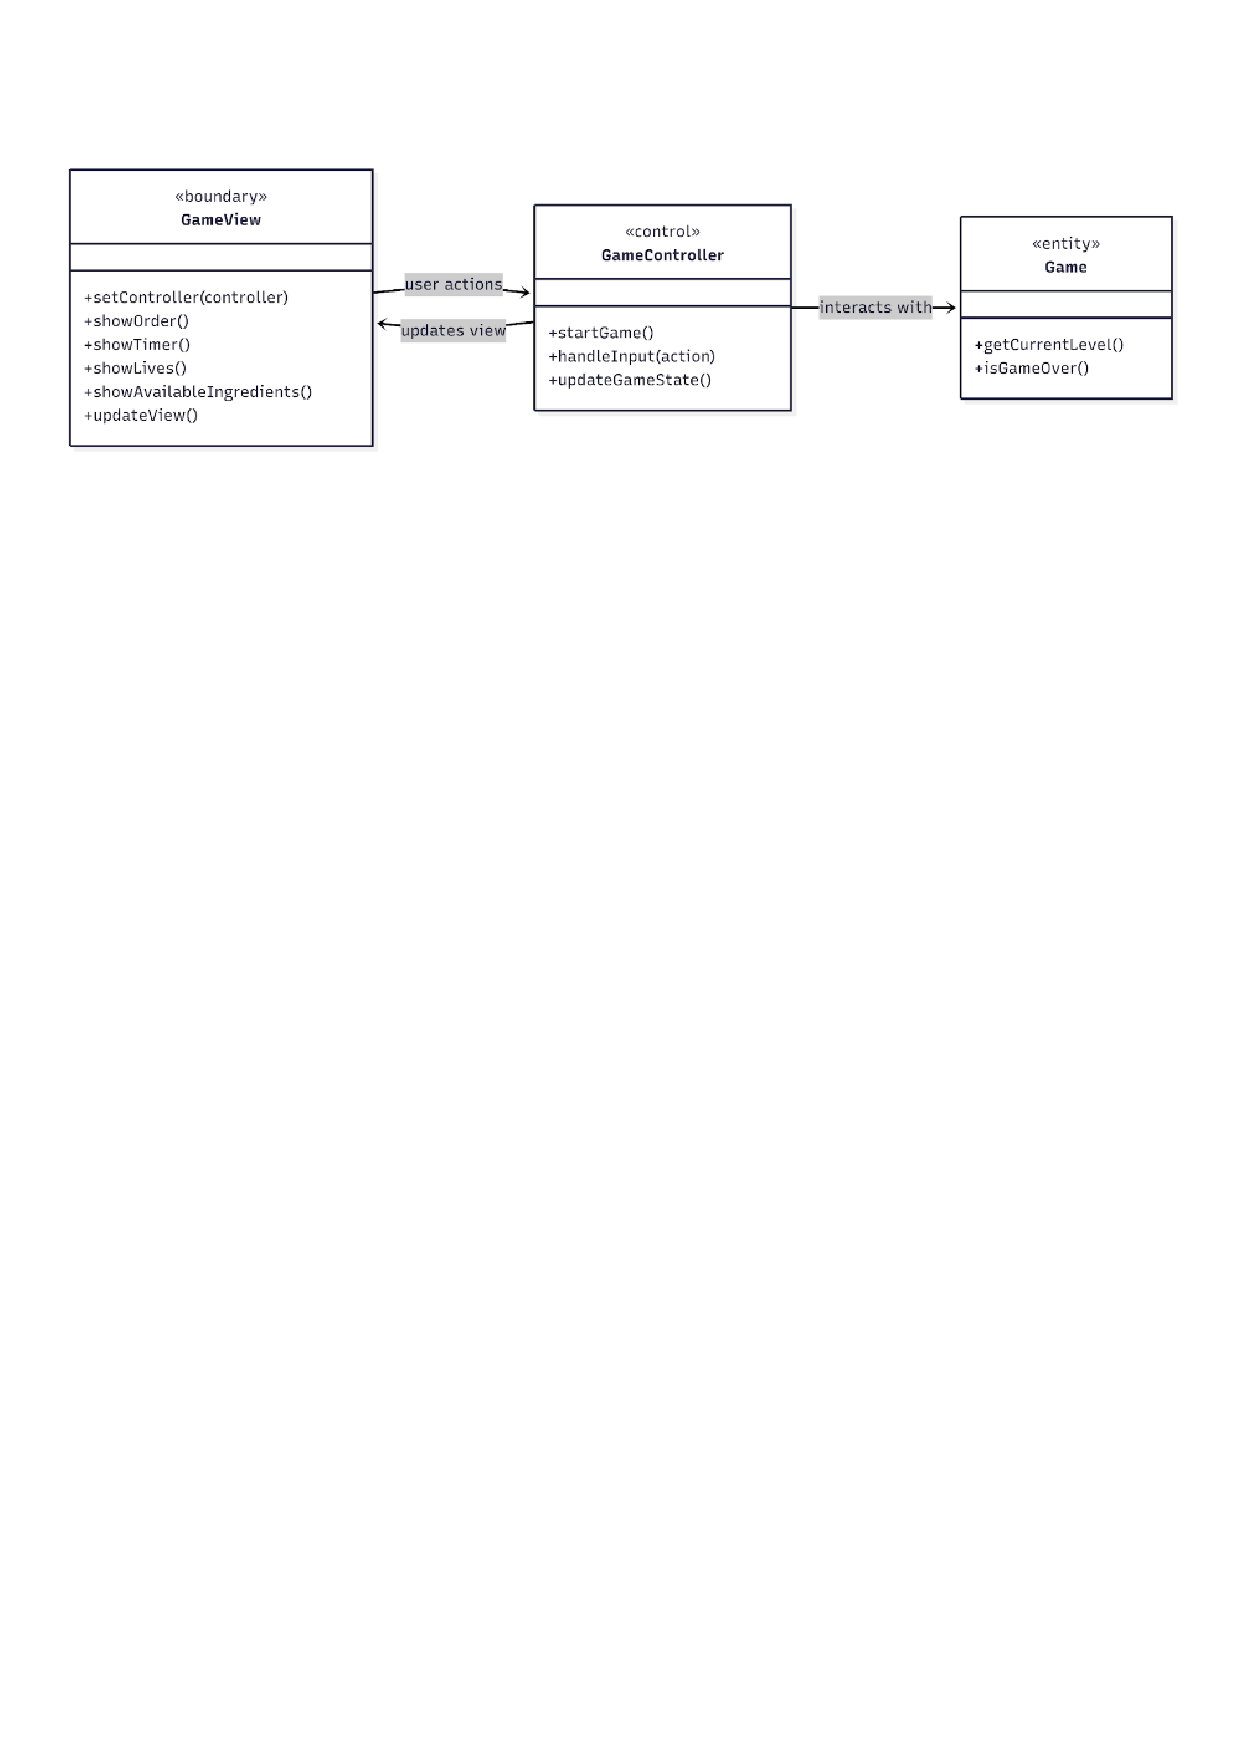
\includegraphics[width=\textwidth, trim=0 20cm 0 0, clip]{img/UML_Architecture.pdf} %prime ricerca su google per tagliare immagini, https://guitex.org/home/en/forum/5-tex-e-latex/49574-risolto-tagliare-le-immagini
%    \caption{Schema UML architetturale di Make an Ice Cream. L’interfaccia \texttt{GameController} è il controller del sistema, e coordina le interazioni tra le interfacce \texttt{GameView} e \texttt{Game}.}
%    \label{img:Architecture}
%\end{figure}


\section{Design dettagliato}

\subsection{Sophy Mercuri}
Questa sezione descrive il design relativo definendo le principali responsabilità e interazioni riguardanti la gestione dei clienti (customer), degli ordini (order) e del timer che gestisce i tempi di attesa dei clienti (CustomerTimer).

%\begin{figure}[H]
%    \centering
%    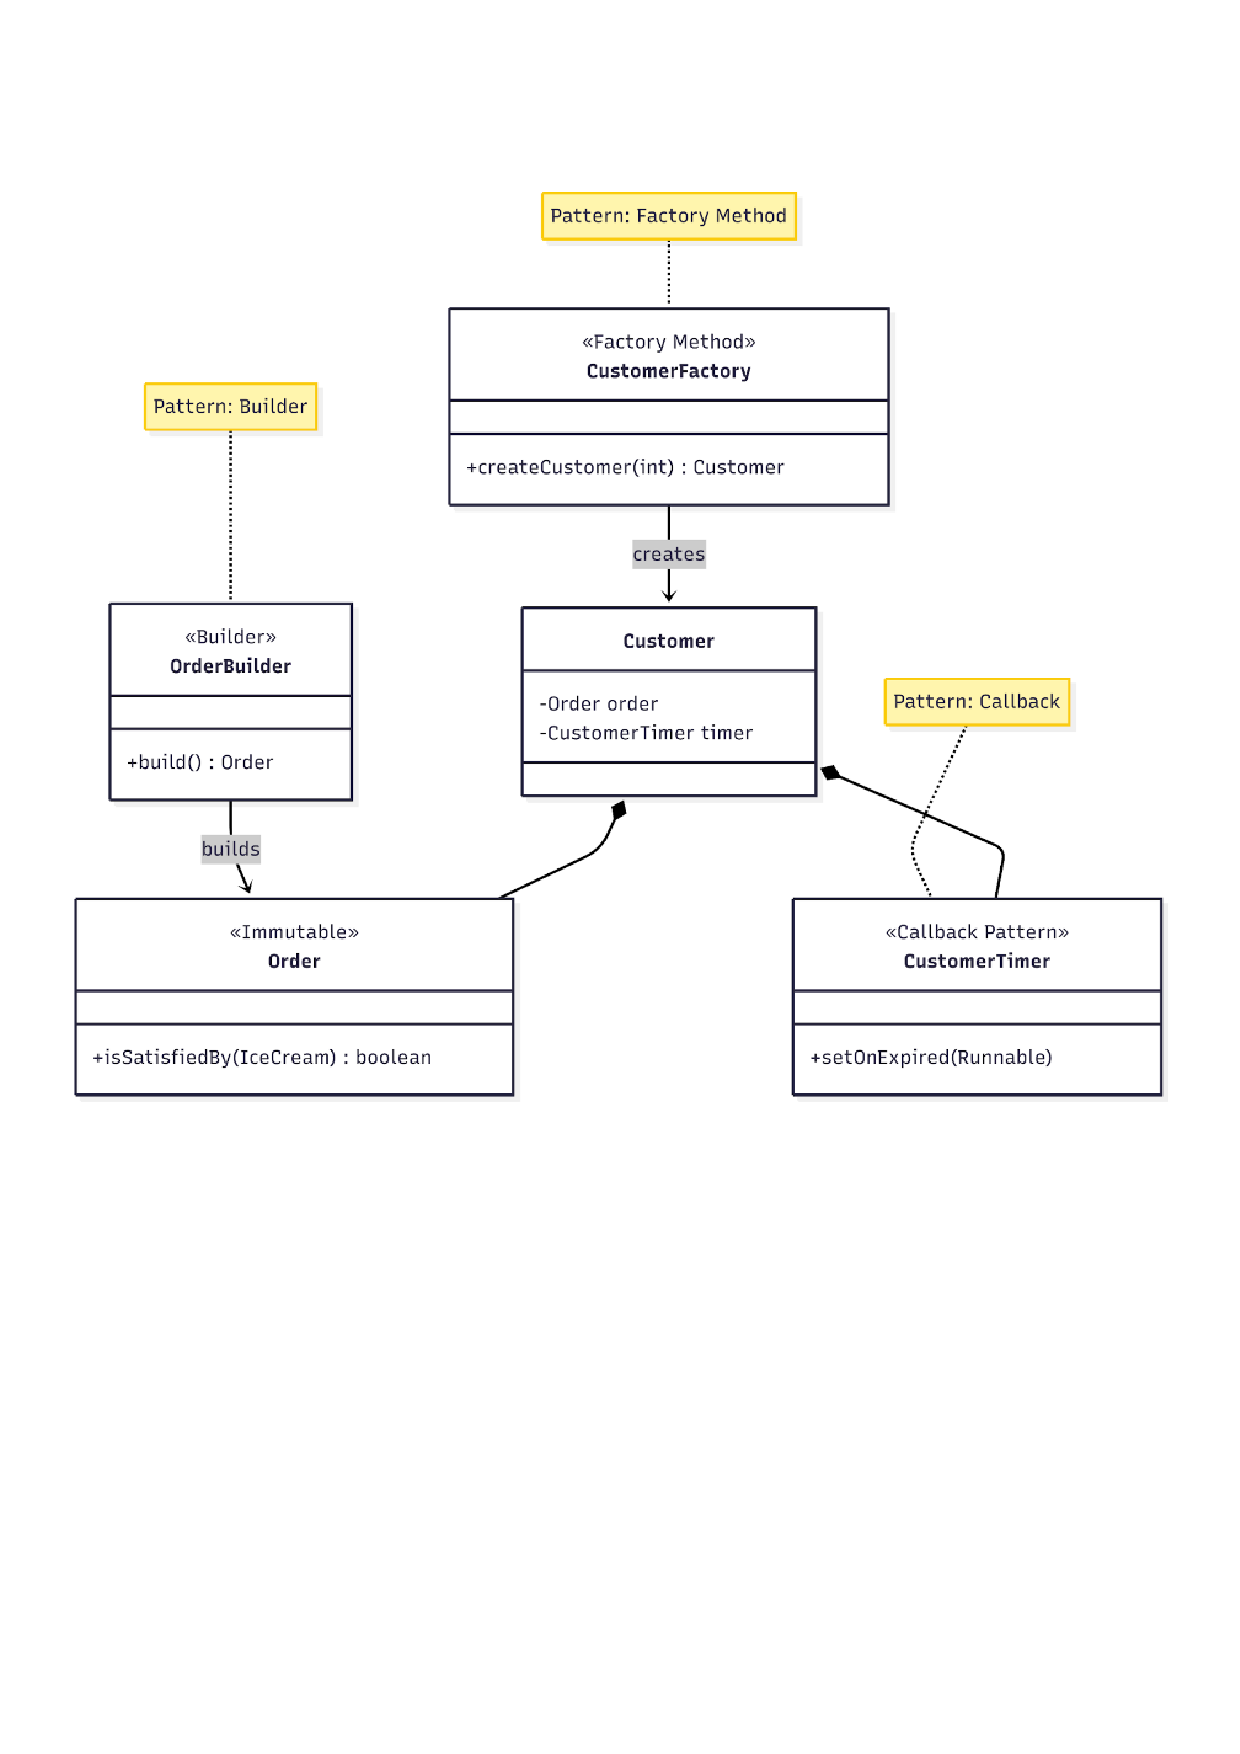
\includegraphics[width=\textwidth, trim=0 10cm 0 2cm, clip]{img/UML_Customer.pdf}
%    \caption{Schema UML relativo a Customer}
%    \label{img:UML_Customer}
%\end{figure}

\subsubsection{Creazione dei clienti che possiedono un ordine}
\paragraph{Problema}
Nel gioco ci sono diverse tipologie di clienti. Ogni cliente ha:
\begin{itemize}
    \item Un nome (scelto casualmente da una lista)
    \item Una difficoltà specifica per la composizione del gelato (mappata al nome)
    \item Un ordine da richiedere, generato casualmente ma sensato ai parametri stabiliti
    \item Un callback da attaccare al timer
\end{itemize}

\paragraph{Responsabilità da rispettare riguardanti il cliente}
\begin{itemize}
    \item Avere una difficoltà definita e associata al suo nome
    \item Disponere di un attributo Order la cui composizione non sia di difficoltà maggiore a quella proporzionata dal livello
    \item Disponere di un attributo Customer Timer
    \item Callback configurato che notifica la scadenza del timer del cliente
\end{itemize}

\paragraph{Approccio per la soluzione}
Usare il pattern ``FACTORY''.
Perchè? Ci permette incapsulare tutta la logica di creazione dei clienti in un unico punto: \texttt{CustomerFactory}. Essa utilizza internamente una classe \texttt{CustomerTemplate} per definire le configurazioni base delle diverse difficoltà di modo che se in futuro voglio andare ad aggiungere un cliente basato su una nuova difficoltà so dove andare. Separazione delle responsabilità, il controller non deve sapere esattamente come si fabbrica un cliente. Deve solo chiedere che gli venga dato un in base alla difficoltà da lui proporzionata. Testabilità, ci permette di testare la factory indipendentemente dal reso del gioco, verificando che i clienti siano stati generati rispettando sempre le regole.

Cosa accade dentro la factory, una volta ricevuta la difficoltà:
\begin{enumerate}
    \item Viene scelto un nome casuale (non mappato a una difficoltà minore)
    \item Gli viene impostato il tempo limite definito dal livello per la difficoltà passata
    \item Genera un ordine casuale: Sceglie un cono, sceglie da 1 a ... riceve un parametro di difficoltà (dal livello corrente) e restituisce un cliente con una configurazione completa.
\end{enumerate}
Ci permette in modo che se domani voglio aggiungere una nuova difficoltà per il profilo di un cliente nuovo, so esattamente dove andare. Separazione delle responsabilità, perchè il controller non deve sapere come si fa un cliente, ma deve solo chiedere un cliente in base alla difficoltà che proporziona modo che in \texttt{CustomerFactory.createCustomer()} in modo che questo riceva un intero (\texttt{maxDifficulty}) che rappresenti la difficoltà del livello in cui si troverà il cliente, in base a questo si crea un cliente di difficoltà equivalente a quella passata o inferiore. Testabilità.

%\begin{figure}[H]
%    \centering
%    \includegraphics[width=\textwidth, trim=0 10cm 0 2cm, clip]{img/UML_CustomerFactory.pdf}
%    \caption{Schema UML relativo alla Factory}
%    \label{img:UML_Factory}
%\end{figure}

\subsubsection{Gestione degli ordini e validazione del gelato}
\paragraph{Problema}
Un ordine (\texttt{Order}) è un oggetto la cui complessità è determinata da tipologia del cliente che effettua l’ordine può essere composto da:
\begin{itemize}
    \item Una lista di gusti (1 elemento min - max 3)
    \item Un cono (obbligatorio)
    \item Una lista di topping (0-2 elementi)
\end{itemize}

Seguendo le regole di dominio imposte:
\begin{itemize}
    \item I gusti devono essere di tipo SCOOP
    \item I topping devono essere LIQUID o SOLID
    \item Massimo un topping SOLID per ordine (non ci possono essere topping solidi tra gli SCOOP)
    \item Non si possono aggiungere ingredienti dopo un topping solido
\end{itemize}

\paragraph{Responsabilità da rispettare}
Costruire un ordine e memorizzarlo correttamente rispettando i parametri di dominio. Verificare se un gelato composto dal giocatore soddisfa la richiesta del cliente.

\paragraph{Approccio per la soluzione}
Usare il pattern ``BUILDER''.
Perchè? Ci favorisce nel controllo. La classe \texttt{OrderBuilder} si occupa di costruire l’ordine ad ogni passo, controllando a sua volta che tutte le regole siano rispettate, che i tipi siano corretti e che non ci siano null, e preserva l’ordine della sequenza con cui è stato costruito il gelato. Il pattern Builder favorisce la comprensione, poiché le operazioni di stanziamento sono eseguite in sequenza. \texttt{OrderImpl} che implementa l'interfaccia \texttt{Order}, proporziona la rappresentazione dell'ordine in modo immutabile, verifica che i SOLID\_TOPPING non siano maggiori a uno.

La verifica dell’ordine all'interno di \texttt{OrderImpl} la preservazione della sequenza esatta degli ingredienti del Order creato ci permette attraverso il metodo \texttt{isSatisfiedBy()} di confrontare l’\texttt{IceCream} creato dal Player (passato come parametro) e l’\texttt{Order} creato in \texttt{OrderBuilder}. L'esito positivo del confronto comprende che:
\begin{itemize}
    \item Abbiano lo stesso cono
    \item Abbiano gli stessi gusti, nello stesso ordine
    \item Abbiano gli stessi topping, nello stesso ordine
\end{itemize}
Per garantire questo, inizialmente si verifica che il gelato passato non sia di tipo null, che sia uguale il tipo di cono (cone), poi si verifica che le lunghezze di entrambe liste sia uguale e la corrispondenza di ogni flavor e topping, posizione per posizione avvantaggiandosi delle liste di tipo \texttt{Ingredient}: con hashcode ed equal ridefinito logicamente per i topping e i flavor (dallo studente 2) in modo di poter verificare facilmente le liste corrispondente al Order e all'Ice Cream.

%\begin{figure}[H]
%    \centering
%    \includegraphics[width=\textwidth, trim=0 10cm 0 2cm, clip]{img/UML_Order.pdf}
%    \caption{Schema UML relativo agli Ordini}
%    \label{img:UML_Order}
%\end{figure}

\subsubsection{Gestione del timer}
\paragraph{Problema Generale}
Il gioco richiede che ogni cliente abbia un timer il cui tempo rappresenti il limite di “pazienza” per ricevere il gelato. Al verificarsi lo scadere del tempo il giocatore perde una vita e il cliente non è soddisfatto. Il timer deve:
\begin{itemize}
    \item Contare alla rovescia in modo preciso
    \item Poter essere messo in pausa e ripreso
    \item Notificare quando il suo tempo è scaduto
\end{itemize}

\paragraph{Problema organizzativo}
Coordinare l'implementazione timer alla presa di decisione dagli studenti incaricati:
\begin{itemize}
    \item Di gestire il flusso di gioco: studente 4 (avviare, fermare, mettere in pausa)
    \item Dell’Implementazione delle regole di gioco, specificamente decidere cosa fare allo scadere del timer: studente 3 (togliere una vita, finire la partita, ecc)
\end{itemize}
Complicando come si sarebbe gestita la scadenza, lasciando un bisogno di modellare un timer che assumesse successivamente comportamenti specifici davanti a certe situazioni senza basarsi in metodi in costruzioni o soggetti a cambi.

\paragraph{Approccio per la soluzione}
``CALLBACK'' con setter.
Si è implementato il timer in modo che sapesse semplicemente contare. Il timer è stato creato con l’incertezza di cosa succede esattamente alla sua terminazione. Sa solo che, allo scadere del tempo, questo dovrà eseguire un comportamento che è stato passato dall’esterno, specificamente con un setter, non nel costruttore. Questo col proposito di favorire il lavoro in parallelo, semplificando l’implementazione e dando l’autonomia ai miei compagni di decidere come proseguere o fare cambiamenti.

\paragraph{Approccio per la soluzione al problema generale}
``Observer'' (minimale):
Invece dell'implementazione delle interfaccia Observer e Observable, la lista di observer e i conseguenti metodi per aggiungere o rimuovere un observer della lista, o notificare tutti si è implementato uno minimale con:
\begin{itemize}
    \item Zero interfacce (si è usato un Runnable di Java)
    \item Un solo observer per il timer
    \item Un solo metodo per impostarlo
    \item Una notifica che va a uno solo e non una lista
\end{itemize}
Perchè? Nel nostro gioco, ogni timer ha esattamente un osservatore. Il cliente ha un timer, e quando quel timer scade deve avvisare il cliente (o il livello, o il controller). Non serve una lista, non serve rimuovere dinamicamente, non serve notificare dieci componenti diversi.

Vantaggi concreti di questa soluzione:
\begin{itemize}
    \item \textbf{Testabilità}: Posso testare il timer senza dover creare un controller, un livello, un cliente o una finestra Swing. Creo un timer, gli passo un callback finto che si limita a settare una variabile booleana, simulo il passare del tempo e verifico che il callback venga chiamato. Pulito, veloce, isolato.
    \item \textbf{Flessibilità}: Lo stesso identico timer può essere usato per diverse parti (Clienti normali, Clienti speciali, Tutorial, Modalità allenamento). Cambia solo il callback, il timer è sempre lo stesso.
\end{itemize}



\subsection{Shuyi Zhang}
\subsubsection{Costruzione del gelato}
\paragraph{Problema}
Il sistema deve creare e gestire istanze di gelato in due situazioni diverse:
\begin{itemize}
    \item Generare una preview del gelato richiesto dal cliente a partire dall’Order;
    \item Gestire il gelato costruito dal giocatore in modo incrementale (scelta cono + aggiunta ingredienti).
\end{itemize}
In entrambi i casi è necessario rispettare gli stessi vincoli di dominio e di gioco (ad esempio numero massimo di gusti, disponibilità di ingredienti legata al livello, combinazioni ammissibili). Senza una soluzione dedicata, la logica di costruzione rischia di essere duplicata tra ordine e interazione utente, rendendo più difficile mantenere coerenza ed evolvere le regole.

\paragraph{Soluzione}
La costruzione del gelato viene centralizzata in \texttt{IceCreamBuilder}, come mostrato in \Cref{img:UML_IceCreamBuilder}.
Il builder incapsula:
\begin{itemize}
    \item La composizione di un gelato come combinazione di Cone e lista Ingredient;
    \item L’applicazione dei vincoli durante la creazione (o durante gli aggiornamenti incrementali).
\end{itemize}
L’Order non costituisce direttamente oggetti complessi, che delega al builder la creazione del gelato di preview del cliente. In modo analogo, la costruzione interattiva del giocatore utilizza lo stesso builder per aggiornare coerentemente lo stato coerente.
Questa scelta riduce duplicazione, garantisce uniformità delle regole e semplifica l’introduzione di nuovi vincoli o ingredienti.
Abbiamo usato in questo caso il pattern Builder, per centralizzare la logica di costruzione e rendere riusabile lo stesso processo sia nella generazione della preview dell’ordine sia nella costruzione incrementale guidata dall’utente.

\begin{figure}[H]
    \centering
    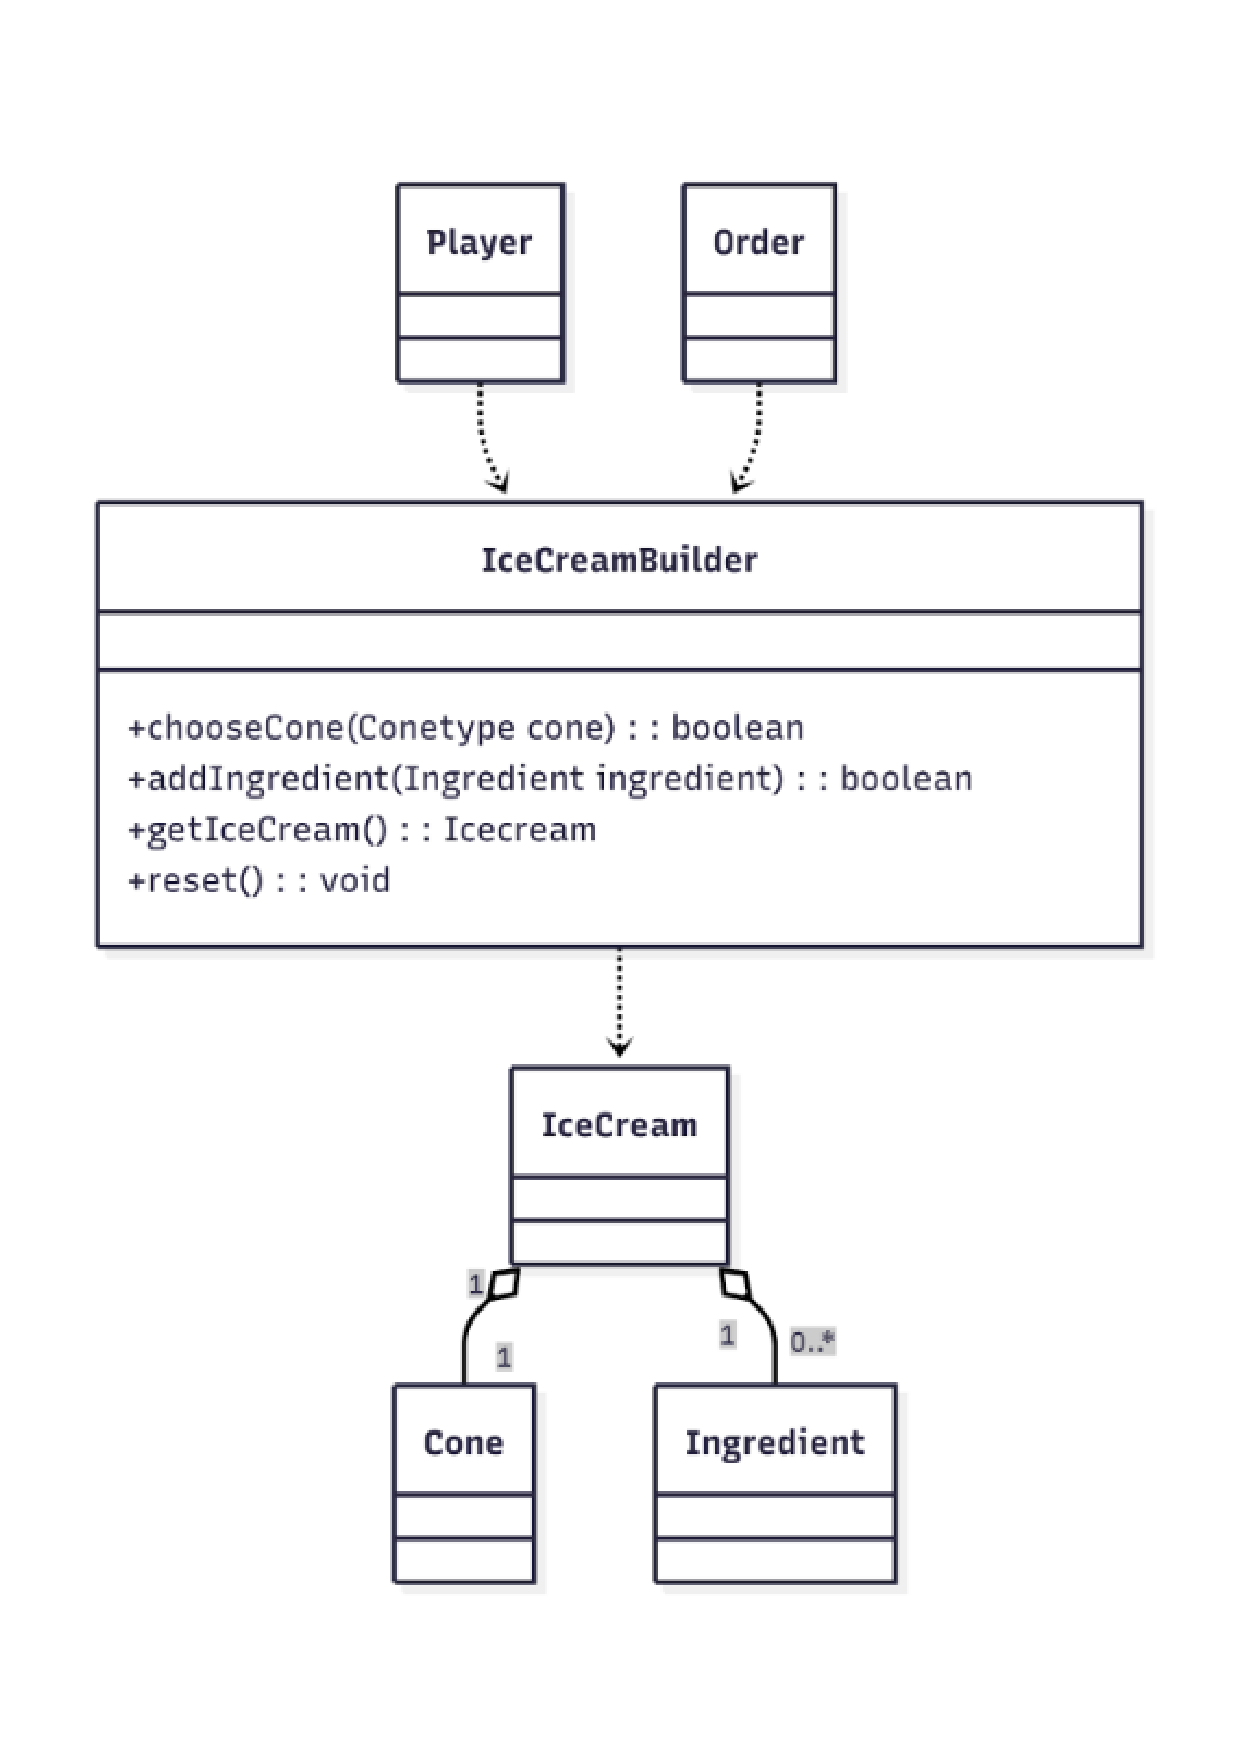
\includegraphics[width=\textwidth, trim=0 2cm 0 0, clip]{img/UML_IceCreamBuilder.pdf}
    \caption{Schema UML relativo al Builder}
    \label{img:UML_IceCreamBuilder}
\end{figure}

\subsubsection{Modellazione degli ingredienti del gelato}
\paragraph{Problema}
Il gelato può includere ingredienti differenti (palline di gusto, topping liquidi, topping solidi). Il sistema deve rappresentarli in modo uniforme e tipizzato, mantenendo l’estendibilità e prevenendo l’uso di valori non validi (es. stringhe arbitrarie per gusti o topping).

\paragraph{Soluzione}
Gli ingredienti condividono l’astrazione \texttt{Ingredient}, con implementazioni concrete per le diverse categorie. Inoltre, gusti e tipologie di topping sono rappresentati tramite enumerazioni dedicate, vincolando i valori ammessi dal dominio e mantenendo il modello consistente.
Il gelato e il builder interagiscono esclusivamente con l’astrazione \texttt{Ingredient}, permettendo di gestire in modo polimorfico tutti i componenti del gelato e di aggiungere nuove tipologie senza modificare la struttura esistente.
Questa scelta migliora l’estendibilità del modello e riduce l’accoppiamento tra le componenti.

\begin{figure}[H]
    \centering
    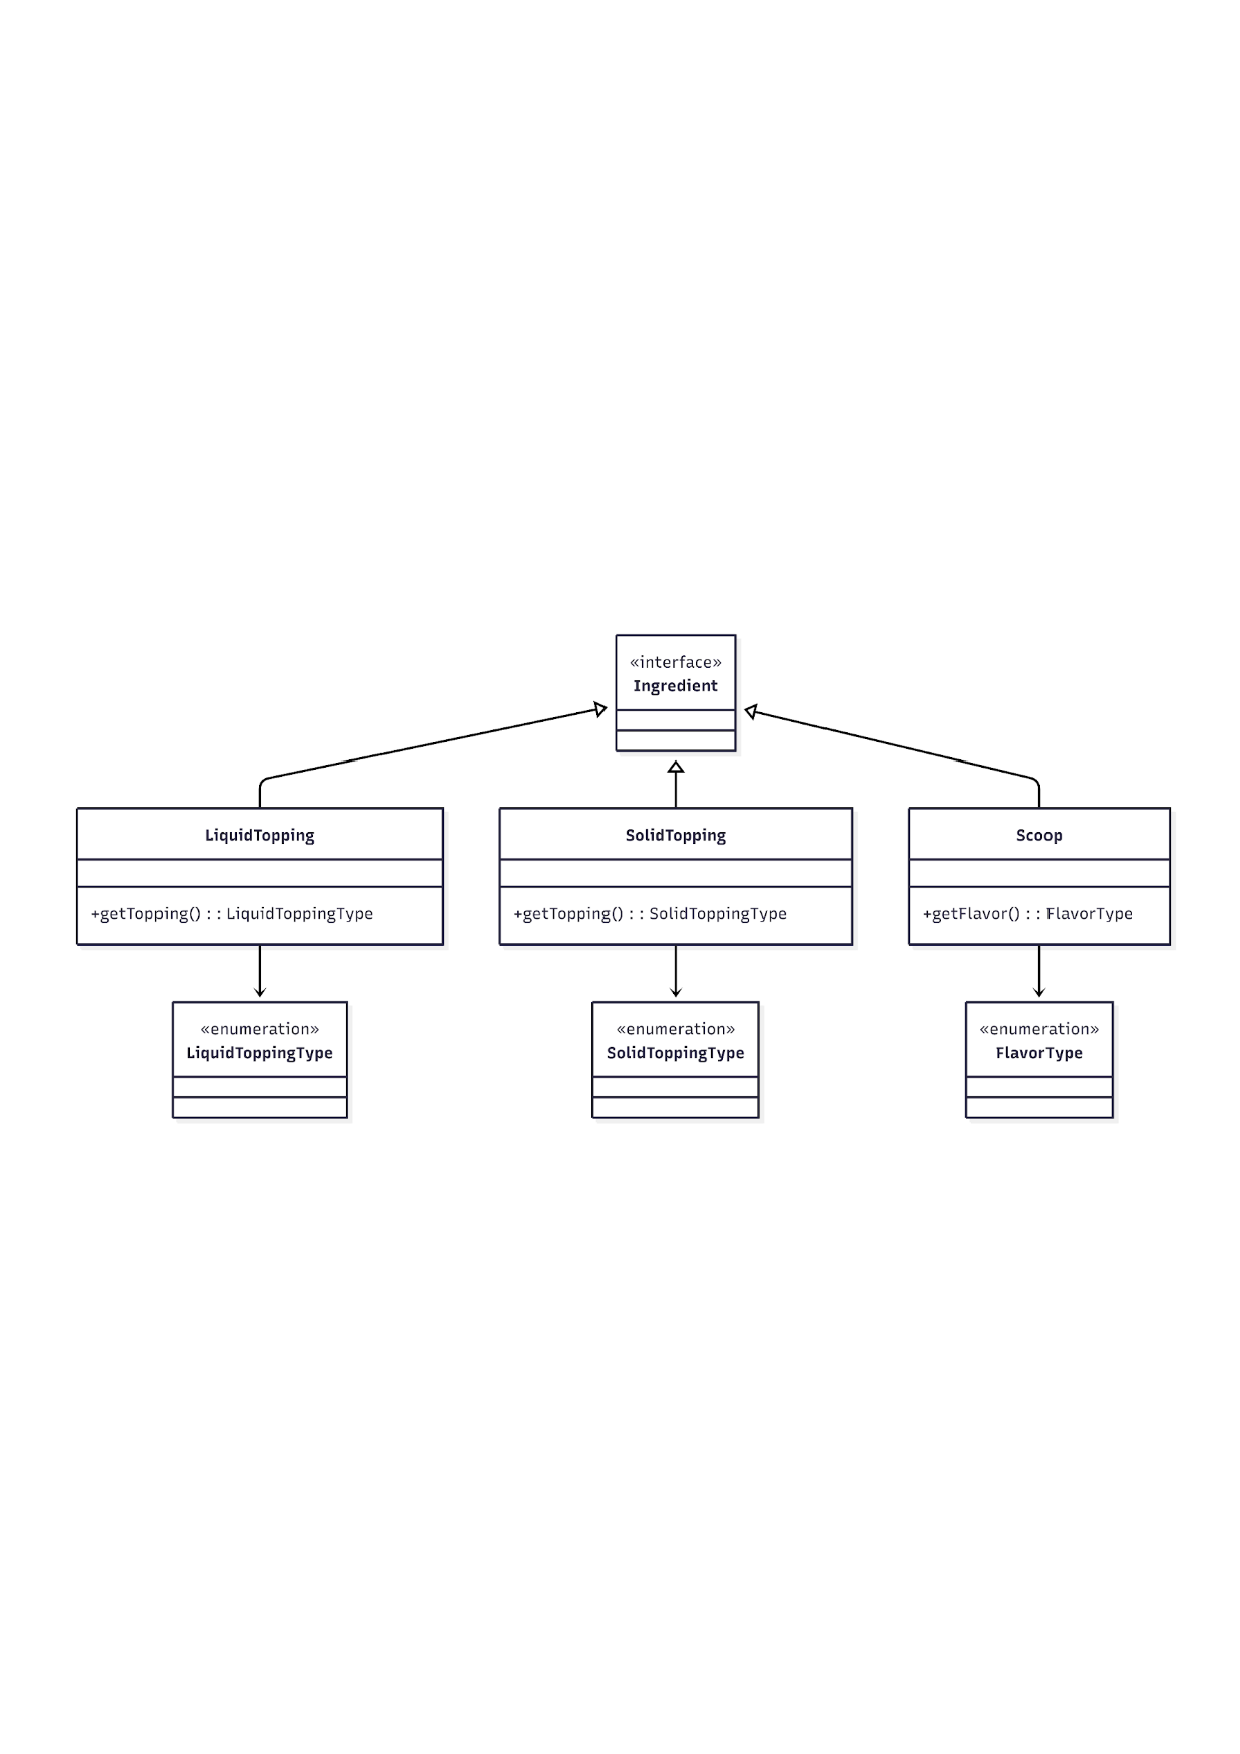
\includegraphics[width=\textwidth, trim=0 10cm 0 10cm, clip]{img/UML_Ingredients.pdf}
    \caption{Schema UML relativo agli Ingredienti}
    \label{img:UML_Ingredients}
\end{figure}

\subsubsection{Costruzione progressiva}
\paragraph{Problema}
Il gelato è composto da diversi ingredienti variabili (base/cono, gusto, topping). Preparare tutti gli elementi contemporaneamente risulta scomodo e poco flessibile. Un approccio più naturale consiste nel prepararlo in modo progressivo, aggiungendo un ingrediente alla volta, proprio come in una gelateria (tramite click del giocatore). Alcuni ingredienti seguono regole precise: i gusti possono essere aggiunti più volte; i topping liquidi possono essere aggiunti tra due gusti; mentre i topping solidi possono essere aggiunti solo una volta ed esclusivamente sopra, una volta; l’aggiunta di un topping solido rappresenta una stato terminale che chiude il gelato e impedisce ulteriori modifiche; inoltre i topping vengono disabilitati nei primi livelli; una base può contenere al massimo tre palline.
(Inoltre, per ogni cliente il gioco deve generare un gelato che chiamiamo “target” a partire dall’ordine e confrontarlo con il gelato effettivamente costruito dal giocatore tramite click.)

\paragraph{Soluzione}
Per la costruzione del gelato viene utilizzato il Builder Pattern. Il gelato è un oggetto composto da più parti (cono, sequenza di gusti, topping) e viene creato in modo progressivo, un ingrediente alla volta. Il builder centralizza la logica di costruzione e applica in un unico punto i vincoli del gioco, ad esempio: massimo tre palline, disponibilità dei topping in base al livello, e chiusura del gelato dopo l’aggiunta di un topping solido (dopo la quale non è più possibile modificare il gelato).
Questa scelta rende il modello più chiaro e riduce il rischio di duplicare le regole di controller e view, mantenendo il processo di creazione ordinato e facilmente estendibile.
Il builder viene utilizzato in due contesti diversi ma con la stessa logica, garantendo coerenza tra ciò che richiede il cliente e ciò che costruisce il giocatore.
\begin{itemize}
    \item \textbf{Gelato target (cliente)}: l’ordine del cliente fornisce una ricetta composta da tipo di cono, lista di gusti e lista di topping. Il builder interpreta questa ricetta e conosce un’istanza di \texttt{IceCream} che rappresenta il gelato target da imitare. In questo modo la figura del cliente è ottenuta applicando la stessa logica e gli stessi vincoli previsti dal gioco.
    \item \textbf{Gelato del giocatore}: il gelato del giocatore viene costruito progressivamente tramite click sugli ingredienti. Ogni click corrisponde a una richiesta di aggiunta (gusto o topping) gestita dal builder, che verifica i vincoli e aggiorna lo stato del gelato. Se viene aggiunto un topping solido, il gelato entra nello stato terminale di chiusura e non sono più consentite ulteriori aggiunte.
\end{itemize}
Al termine, il gelato del giocatore viene confrontato con il gelato target verificando che la configurazione finale coincida, determinando l’esito dell’ordine.
Una possibile alternativa sarebbe stata gestire la costruzione del gelato come semplice modifica di liste direttamente nel controller o nella view (ad esempio aggiungendo/rimuovendo elementi e controllando manualmente i vincoli). Questa soluzione è più immediata, ma presenta lo svantaggio di distribuire la logica in più punti del codice, rendendo più probabili incoerenze e rendendo più difficile il testing.
Un’ulteriore alternativa sarebbe stata adottare il Decorator Pattern, modellando ogni ingrediente come uno strato che avvolge lo stato precedente. Sebbene questa soluzione rappresenti bene l’idea di stratificazione, nel contesto del gioco risulta meno pratica per il confronto tra gelato target e gelato del giocatore e per la gestione di regole legate al livello. Inoltre, introduce un numero maggiore di classi e una struttura più complessa.

\subsection{Gestione del Giocatore e Livelli (Studente 3)}

\subsubsection{Gestione del giocatore e della consegna degli ordini}

\paragraph{Problema}
Nel gioco Make an Ice Cream il giocatore è l’entità che interagisce attivamente con il sistema: costruisce un gelato e lo consegna al cliente corrente.
Il sistema deve:
\begin{itemize}
    \item Rappresentare il giocatore come entità autonoma del modello.
    \item Gestire l’azione di consegna del gelato.
    \item Produrre un esito dell’ordine che possa influenzare lo stato del livello (avanzamento o perdita di una vita).
\end{itemize}

\paragraph{Soluzione}
Il giocatore è modellato nella classe \texttt{Player}, che incapsula le azioni principali disponibili durante il gioco.
In particolare, il metodo \texttt{deliverIceCream(...)} rappresenta la consegna del gelato al cliente corrente.
Il \texttt{Player} non gestisce direttamente le regole di gioco (vite, progressione o clienti), ma si limita a:
\begin{itemize}
    \item Ricevere il gelato costruito dal giocatore.
    \item Inoltrare la consegna al cliente corrente.
    \item Ricevere l’esito dell’operazione dal cliente.
\end{itemize}
Il livello utilizza tale esito per aggiornare il proprio stato, consentendo una separazione netta tra l'azione del giocatore (\texttt{Player}) e le regole del gioco (\texttt{Level}).
Questa scelta mantiene il modello modulare e favorisce il riuso del codice, evitando che la logica della consegna venga duplicata o sparsa in componenti non appropriati.\Cref{img:UML_Level}.

\begin{figure}[H]
    \centering
    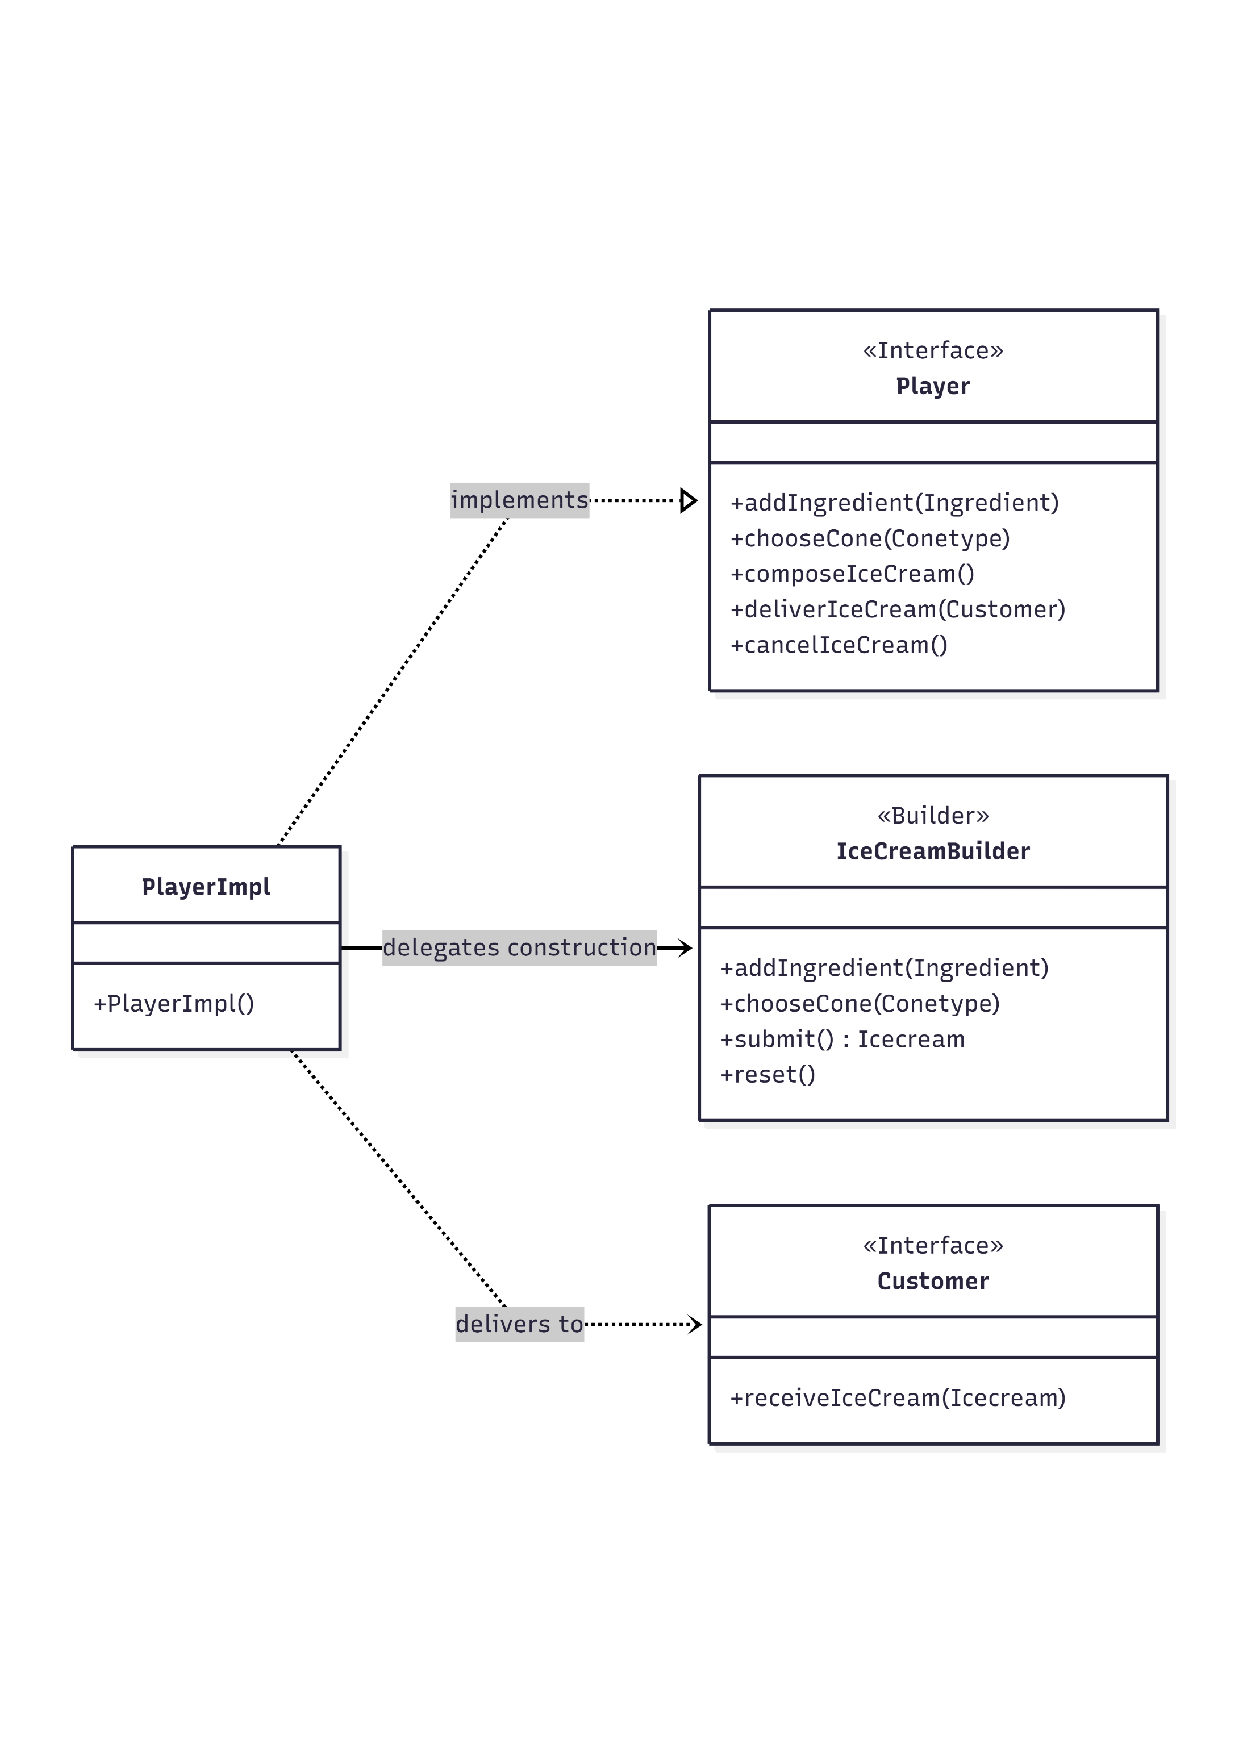
\includegraphics[width=\textwidth, trim=0 5cm 0 5cm, clip]{img/UML_Player.pdf}
    \caption{Schema UML del giocatore, con rappresentate le entità principali ed i rapporti fra loro}
    \label{img:UML_Player}
\end{figure}
\subsubsection{Gestione dei livelli e progressione della difficoltà}

\paragraph{Problema}
Il gioco Make an Ice Cream è strutturato in livelli a difficoltà crescente.
Prima dell’inizio della partita il giocatore seleziona un livello, ma il sistema deve:
\begin{itemize}
    \item Creare un livello coerente con la difficoltà scelta.
    \item Inizializzare correttamente vite, numero di clienti e parametri di gioco.
    \item Garantire una progressione graduale della difficoltà.
    \item Mantenere la logica di creazione e gestione del livello separata dal controller e dalla view.
\end{itemize}

\paragraph{Soluzione}
Per la gestione dei livelli è stato utilizzato il pattern \textit{Simple Factory}. Prima dell’inizio del livello il giocatore seleziona un valore intero compreso tra 1 e 5, che rappresenta il livello scelto. Questo valore viene poi utilizzato come parametro di difficoltà passato alla factory per la creazione del livello.
Il livello creato gestisce le vite disponibili e la sequenza di clienti, a cui è stato propagato il parametro di difficoltà che influenza la complessità degli ordini e i tempi di attesa dei clienti, garantendo una progressione graduale di difficoltà.
L’uso del factory consente di centralizzare la logica per poi evitare duplicazioni necessarie future per estendere il gioco introducendo nuove tipologie di livelli.\Cref{img:UML_Level}.

\begin{figure}[H]
    \centering
    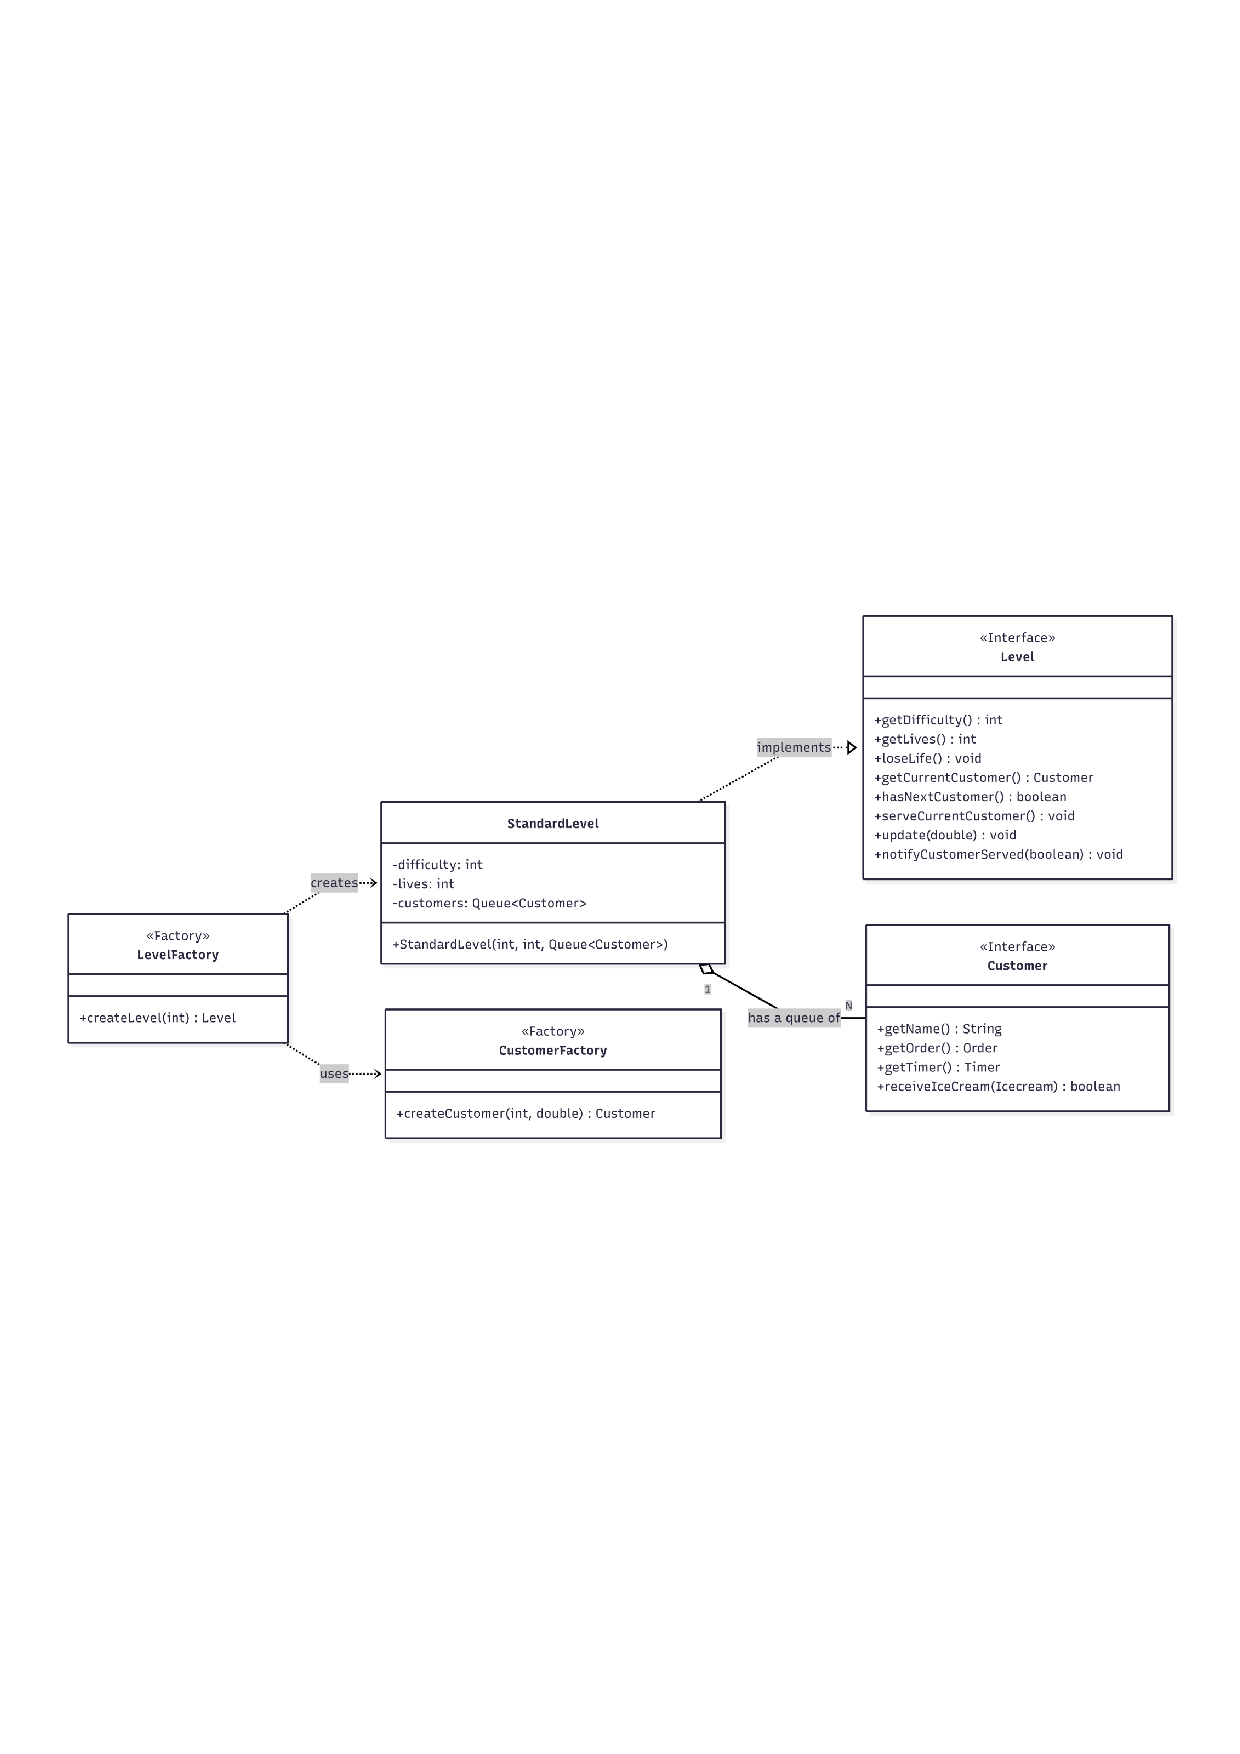
\includegraphics[width=\textwidth, trim=0 10cm 0 10cm, clip]{img/UML_Level.pdf}
    \caption{Schema UML del livello, con rappresentate le entità principali ed i rapporti fra loro}
    \label{img:UML_Level}
\end{figure}

\subsection{Chiara Emina}
\subsubsection{Gestione dei comandi utente}
\paragraph{Problema}
Il controller del gioco deve gestire tutte le possibili azioni dell’utente, e il sistema deve permettere di aggiungere nuovi comandi in futuro senza modificare il controller esistente.

\paragraph{Soluzione}
Il sistema per la gestione dei comandi utilizza il pattern Command, come da Figura … : ogni azione del gioco è rappresentata da un oggetto Command che incapsula la logica specifica dell’azione e delega l’esecuzione di essa al modello Game, che funge da receiver. Il controller, ovvero GameControllerImpl, agisce invece da invoker, creando ed eseguendo il comando corrispondente all’azione ricevuta, senza però saperne l’implementazione. In questo modo, nuove azioni possono essere aggiunte creando semplicemente un nuovo comando e mantenendo il controller semplice e leggibile. A titolo esemplificativo, in Figura …, AddIngredientCommand e DeliverCommand mostrano come un comando concreto implementa l’interfaccia Command e interagisce con il modello.


%\begin{figure}[H]
%    \centering
%    \includegraphics[width=\textwidth, trim=0 10cm 0 10cm, clip]{img/UML_Command.pdf}
%    \caption{Rappresentazione UML del pattern Command per la gestione delle azioni dell’utente.}
%    \label{img:UML_Command}
%\end{figure}

\subsubsection{Gestione degli eventi utente}

%\begin{figure}[H]
%    \centering
%    \includegraphics[width=\textwidth, trim=0 10cm 0 10cm, clip]{img/UML_Event.pdf}
%    \caption{Rappresentazione UML di GameAction. L’interfaccia GameAction definisce il tipo di azione dell’utente, GameActionImpl ne fornisce l’implementazione concreta, mentre GameActionType elenca tutti i possibili tipi di azione.}
%    \label{img:UML_Event}
%\end{figure}

\paragraph{Problema}
Il sistema deve rappresentare in modo uniforme gli eventi generati dalle azioni dell’utente sull’interfaccia grafica, per permettere al controller di gestirle correttamente senza conoscere i dettagli interni della view.

\paragraph{Soluzione}
Ogni evento è rappresentato da un oggetto EventImpl, che implementa l’interfaccia Event e associa l’azione a un valore dell’enumerazione Eventype, come mostrato in Figura …. In questo modo il controller può interrogare il tipo di azione e creare il comando corrispondente senza preoccuparsi della logica interna. Questo design consente al controller di gestire tutti gli eventi in modo uniforme e può essere facilmente esteso per supportare nuovi tipi di eventi.


\subsubsection{Gestione dello stato del gioco}

%\begin{figure}[H]
%    \centering
%    \includegraphics[width=\textwidth, trim=0 10cm 0 10cm, clip]{img/UML_GameState.pdf}
%    \caption{Rappresentazione UML della gestione dello stato in GameImpl. L’enumerazione GameState definisce i possibili stati del gioco, mentre GameImpl li utilizza per gestire transizioni come avvio, pausa, ripresa e ritorno al menu.}
%    \label{img:UML_GameState}
%\end{figure}

\paragraph{Problema}
Il sistema deve tenere traccia dello stato corrente del gioco e gestire correttamente transizioni come avvio di un livello, pausa e ripresa, fine livello o game over.

\paragraph{Soluzione}
Come mostrato in Figura …, GameImpl utilizza l’enumerazione GameState per rappresentare lo stato corrente del gioco. Ogni metodo (start(), pause(), resume(), returnToMenu()) modifica lo stato in modo appropriato, mentre update() verifica le condizioni di avanzamento del livello e aggiorna lo stato in base al numero di vite o ai clienti serviti. La scelta di usare un’enumerazione è motivata dalla semplicità del dominio: non vi è un numero elevato di stati ed essi non hanno una complessità tale da dover utilizzare un pattern State, che sarebbe eccessivo per questo caso d’uso.

\subsubsection{Core di gioco}

%\begin{figure}[H]
%    \centering
%    \includegraphics[width=\textwidth, trim=0 10cm 0 10cm, clip]{img/UML_GameEngine.pdf}
%    \caption{Schema UML relativo al GameEngine.}
%    \label{img:UML_GameEngine}
%\end{figure}

\paragraph{Problema}
Il gioco deve aggiornare periodicamente lo stato del modello e notificare la view, senza mescolare logica di esecuzione e gestione degli eventi.

\paragraph{Soluzione}
Il GameCore inizializza il modello (GameImpl) e il controller (GameControllerImpl), e coordina il ciclo principale di esecuzione tramite GameLoop. Il loop calcola il tempo trascorso tra un frame e l’altro e chiama il controller per aggiornare il modello solo se il gioco è in esecuzione. In questo modo la logica del modello e del controller rimane separata dalla gestione del tempo, facilitando estensioni future.



\chapter{Sviluppo}
\section{Testing automatizzato}

\textbf{Player}: sono stati testati la costruzione del gelato in stati validi, la gestione di input non validi e il corretto comportamento della consegna verso il cliente. Mediante oggetti mock è stato verificato l’esito positivo e negativo dell’ordine, controllando anche il reset dello stato interno dopo ogni consegna. È stato inoltre testato l’annullamento della costruzione e la gestione di stati non validi.

\textbf{Level (StandardLevel)}: è stato testato lo stato iniziale del livello (vite, difficoltà, presenza clienti) e la corretta progressione della coda. Sono state verificate la perdita di vite in caso di ordine errato o tempo scaduto e l’aggiornamento temporale tramite timer mockato. È stata inoltre verificata la registrazione e gestione delle callback per propagare l’esito dell’ordine al livello.

\textbf{GameImpl}: Classe che gestisce lo stato della partita, il livello corrente e il giocatore. Definisce le principali operazioni del gioco come l’inizio di un livello, la preparazione del gelato, l’aggiornamento dello stato di gioco e del livello stesso nel tempo. Per questa classe vengono testati la correttezza dello stato iniziale di gioco, l’avvio del livello, le transizioni di stato, la delegazione di azioni al Player e il corretto funzionamento del metodo update(). Per questa classe di test è stato utilizzato un mock di Customer.

\textbf{GameControllerImpl}: Classe che si occupa di coordinare l’esecuzione del gioco collegando modello e view. Gestisce gli input del giocatore trasformandoli in comandi per il model e aggiorna la view in base allo stato di gioco, tenendo traccia di ordini, clienti e vite. Per questa classe si verificano l’impostazione del controller nella view, la gestione degli eventi ricevuti in input e l'esecuzione dei relativi comandi, i controlli dello stato di gioco e l’aggiornamento della view quando il gioco è in stato di playing. In questa classe di test sono stati utilizzati dei mock di Game, GameLoop, GameView, Level ed Event.

\textbf{Classi Command}: Classi che implementano l’interfaccia Command e che rappresentano i possibili comandi di gioco. Per ogni classe è stato effettuato un test che ne verificasse il corretto funzionamento, facendo uso anche in questo caso di diversi mock.

\textbf{GameLoopImpl}: Classe che si occupa di generare il game loop e aggiornare periodicamente il gioco tramite il controller. Per questa classe si sono testati l’avvio e l’arresto del loop tramite l’impostazione della variabile running a true e false, la chiamata ad updater (per il quale si è utilizzato un mock di Consumer), il rispetto dei valori minimo e massimo della variabile elapsed.

\textbf{GameCoreImpl}: Classe che si occupa dell’inizializzazione delle componenti model, controller, view e dell’aggiornamento dello stato di gioco. Per questa classe si è solo verificato che GameCoreImpl esponga correttamente il controller attraverso il metodo getController(). Per farlo, sono stati usati mock di Game, GameController e GameLoop, iniettati tramite il costruttore.
% TODO: Inserire qui le informazioni relative ai test per gli altri componenti

\section{Note di sviluppo}

\subsection{Sophy Mercuri}

\subsection{Shuyi Zhang}

\subsection{Antonio Scharmuller}
\begin{itemize}

\item \textbf{Utilizzo di Lambda expressions} \\
Le lambda expressions sono state utilizzate per registrare dinamicamente le callback tra cliente e livello, permettendo di propagare l’esito dell’ordine in modo compatto e leggibile. L’uso di funzioni come parametro riduce la necessità di classi anonime esplicite e migliora la chiarezza del flusso logico. \\
\textbf{Link:} \url{[PERMALINK StandardLevel -- registrazione callback]}

\item \textbf{Utilizzo di strutture dati della Collections Framework (Queue / ArrayDeque)} \\
La gestione dei clienti nel livello avviene tramite \texttt{Queue} e \texttt{ArrayDeque}, garantendo un comportamento FIFO, consente una gestione efficiente dell’avanzamento del gioco e rende il modello più prevedibile nei test. \\
\textbf{Link:} \url{[PERMALINK StandardLevel -- dichiarazione e utilizzo Queue]}

\item \textbf{Utilizzo di Mockito per il testing} \\
Nei test automatici è stata utilizzata la libreria Mockito per creare mock di \texttt{Customer} e \texttt{Timer}. Questo ha permesso di isolare il comportamento e verificare effetti collaterali e simulare condizioni specifiche (es. scadenza del tempo). \\
\textbf{Link:} \url{[PERMALINK PlayerTest / StandardLevelTest -- utilizzo mock e when/verify]}

\item \textbf{Controllo dello stato tramite validazione esplicita} \\
Sono stati introdotti controlli espliciti su stati non validi (es. consegna senza gelato completo) e su input nulli. Questa scelta migliora la robustezza del modello e previene stati inconsistenti durante l’esecuzione. \\
\textbf{Link:} \url{[PERMALINK PlayerImpl -- controlli su stato e null]}

\end{itemize}

\subsection{Chiara Emina}

\begin{itemize}

\item \textbf{Uso di Lambda expressions} \\
Utilizzate soprattutto in GameControllerImpl per la creazione dei vari comandi. \\
\textbf{Esempio:} \url{https://github.com/Swarz04/OOP25-MakeAnIceCream/blob/a78242d1f39263c851a41fa57e0b26af1d8ecf8f/src/main/java/it/unibo/makeanicecream/controller/GameControllerImpl.java#L52}
\item \textbf{Uso di Method Reference} \\
Utilizzato in GameCoreImpl per passare direttamente il metodo update a GameLoopImpl. \\
\textbf{Esempio:} \url{https://github.com/Swarz04/OOP25-MakeAnIceCream/blob/a78242d1f39263c851a41fa57e0b26af1d8ecf8f/src/main/java/it/unibo/makeanicecream/core/GameCoreImpl.java#L29}
\item \textbf{Uso della libreria Mockito} \\
Utilizzata nelle classi di test, di cui riporto due esempi. \\
\textbf{Esempio:} \url{https://github.com/Swarz04/OOP25-MakeAnIceCream/blob/a78242d1f39263c851a41fa57e0b26af1d8ecf8f/src/test/java/it/unibo/makeanicecream/controller/GameControllerImplTest.java#L44} \\
\textbf{Esempio:} \url{https://github.com/Swarz04/OOP25-MakeAnIceCream/blob/a78242d1f39263c851a41fa57e0b26af1d8ecf8f/src/test/java/it/unibo/makeanicecream/GameImplTest.java#L167}
\item \textbf{Utilizzo del codice del professor Ricci} \\
Per implementare il game loop nella classe GameLoopImpl ho riadattato parti del codice fornito dal professor Alessandro Ricci nel progetto Game-As-A-Lab-Step-00-game-loop. In particolare, ho utilizzato il calcolo del deltaTime (elapsed) e il metodo waitForNextFrame(), riscrivendo e adattando il resto del codice alle esigenze del nostro progetto.

\end{itemize}

\chapter{Commenti finali}

\section{Autovalutazione e lavori futuri}

\subsection{Sophy Mercuri}

\subsection{Shuyi Zhang}

\subsection{Antonio Scharmuller}

\subsection{Chiara Emina}
In questo progetto mi sono occupata della gestione degli stati della partita, del flusso del gioco e dell’integrazione tra i modelli. In particolare, ho sviluppato Game, la classe principale del model che interagisce con il controller e che gestisce la logica principale del gioco. Poi ho implementato il controller garantendo l’integrazione tra model e view e il corretto flusso di esecuzione del gioco attraverso la gestione degli eventi e dei comandi. Ho curato l’aggiornamento della view in base agli eventi del gioco, mostrando informazioni sul cliente corrente, timer, vite e ordini. Inoltre ho implementato il game loop che gestisce il ciclo principale di aggiornamento del gioco.

\begin{itemize}
\item \textbf{Punti di forza} \\
Penso che uno dei principali punti di forza del mio lavoro sia la gestione coerente degli stati della partita e delle loro transizioni, che rende il flusso del gioco chiaro e comprensibile. Ho cercato di curare l’integrazione tra model, controller e view in modo da mantenere una separazione delle responsabilità, favorendo leggibilità e organizzazione del codice. Inoltre, un altro punto di forza penso sia l’utilizzo del pattern Command per la gestione degli eventi, che rende il sistema modulare ed estendibile, permettendo di aggiungere nuove azioni senza modificare in modo invasivo la logica esistente.

\item \textbf{Punti di debolezza} \\
Una probabile debolezza è forse il fatto che il controller è piuttosto centrale e carico di responsabilità, e questo potrebbe essere un limite in termini di scalabilità e manutenibilità. Anche la parte grafica e l’esperienza utente potrebbero essere arricchite con animazioni e maggiore interattività. Inoltre un altro punto di debolezza riguarda la gestione delle schermate nella GameViewImpl, dove la view decide quale pannello mostrare in base al valore dell’enum GameState. Sebbene lo stato venga richiesto tramite il controller, la view rimane comunque a conoscenza di un elemento del dominio del gioco. In futuro si potrebbe rendere la separazione ancora più netta, delegando al controller la responsabilità di indicare direttamente quale schermata visualizzare.
\end{itemize}

\section{Difficoltà incontrate e commenti per i docenti}

\subsection{Sophy Mercuri}

\subsection{Shuyi Zhang}

\subsection{Antonio Scharmuller}

\subsection{Chiara Emina}
La parte più difficile del corso è stata senza dubbio l’esame pratico in laboratorio. Ho avuto grandi difficoltà nella comprensione dell’esercizio di Junit, sia quando ho svolto le prove passate per esercitarmi, sia all’esame, perché ogni volta vi erano diverse entità e meccaniche da implementare che per me erano molto complicate da capire, soprattutto entro un tempo limite. Tuttavia, anche nello svolgimento del progetto ho avuto qualche problema, soprattutto nell’imparare a usare git e a lavorare in gruppo con una data di consegna fissata da rispettare. Queste cose erano tutte nuove per me, e ho trovato qualche difficoltà a gestire le tempistiche di sviluppo del nostro programma, probabilmente anche a causa della mia insicurezza durante la progettazione. Nonostante ciò, grazie a questo progetto ho acquisito familiarità con l’uso di git e con il lavoro di gruppo, e mi sento molto soddisfatta del lavoro realizzato. Penso che questo progetto sia stato un passo molto importante per il mio percorso di studi e crescita personale, soprattutto per quanto riguarda il relazionarsi con altre persone e lavorare insieme.


\appendix
\chapter{Guida utente}

Capitolo in cui si spiega come utilizzare il software. Nel caso in cui il suo uso sia del tutto
banale, tale capitolo può essere omesso.
%
A tal riguardo, si fa presente agli studenti che i docenti non hanno mai utilizzato il software
prima, per cui aspetti che sembrano del tutto banali a chi ha sviluppato l'applicazione possono non
esserlo per chi la usa per la prima volta.
%
Se, ad esempio, per cominciare una partita con un videogioco è necessario premere la barra
spaziatrice, o il tasto ``P'', è necessario che gli studenti lo segnalino.

\subsection*{Elementi positivi}

\begin{itemize}
 \item Si istruisce in modo semplice l'utente sull'uso dell'applicazione, eventualmente facendo uso di schermate e descrizioni.
\end{itemize}

\subsection*{Elementi negativi}
\begin{itemize}
 \item Si descrivono in modo eccessivamente minuzioso tutte le caratteristiche, anche minori, del software in oggetto.
 \item Manca una descrizione che consenta ad un utente qualunque di utilizzare almeno le funzionalità primarie dell'applicativo.
\end{itemize}

\chapter{Esercitazioni di laboratorio}

\subsection{chiara.emina@studio.unibo.it}
\begin{itemize}
 \item Laboratorio 07: \url{https://virtuale.unibo.it/mod/forum/discuss.php?d=207193#p284987}
 \item Laboratorio 08: \url{https://virtuale.unibo.it/mod/forum/discuss.php?d=207921#p286132}
 \item Laboratorio 09: \url{https://virtuale.unibo.it/mod/forum/discuss.php?d=208718#p286856}
 \item Laboratorio 10: \url{https://virtuale.unibo.it/mod/forum/discuss.php?d=209589#p288534}
 \item Laboratorio 11: \url{https://virtuale.unibo.it/mod/forum/discuss.php?d=210617#p289525}
\end{itemize}


\bibliographystyle{alpha}
\bibliography{13-template}

\end{document}
